

\documentclass[8pt]{beamer}
\usetheme{default}
\PassOptionsToPackage{usenames,dvipsnames}{xcolor}
\usepackage{my_pres}
\usepackage{tikz}
\usepackage{empheq,accents}
\usepackage{pifont}
\usetikzlibrary{arrows}



\include{my_header}



\definecolor{texthigh}{RGB}{137, 0, 255}
\definecolor{textred}{RGB}{255, 0, 94}
\definecolor{textgreen}{RGB}{89, 232, 151}
\definecolor{textlightgray}{RGB}{170,170,170}
\definecolor{bggray}{RGB}{230,230,230}
\definecolor{textgray}{RGB}{60,60,60}

\setbeamercolor{background canvas}{bg=bggray}
\setbeamercolor{normal text}{fg=textgray}

\setbeamertemplate{enumerate items}[default]
\setbeamertemplate{itemize items}{\ding{84}}

\title{Improved Estimation of Canonical Vectors in Canonical Correlation Analysis}
\institute[Univ. of Michigan]{Department of Electrical Engineering and Computer
  Science\\University of Michigan\\ }
\author[N. Asendorf, R.R. Nadakuditi]{Nicholas Asendorf, Ph.D. \hspace{10ex} Prof. Raj
  Nadakuditi\\ {\small{\texttt{asendorf@umich.edu} \phantom{addk}\hspace{12ex}
      \texttt{rajnrao@umich.edu}}  }}
\date{Asilomar Conference on Signals, Systems, and Computers\\[2ex] November 11, 2015}

\newcommand{\twr}{{\sf TW}_\reals}
\newcommand{\twc}{{\sf TW}_\complex}
\newcommand{\sx}{s_{x,i}}
\newcommand{\sy}{s_{y,i}}
\newcommand{\zx}{z_{x,i}}
\newcommand{\zy}{z_{y,i}}
\newcommand{\Zx}{Z_x}
\newcommand{\Zy}{Z_y}
\newcommand{\Ux}{U_x}
\newcommand{\Uy}{U_y}
\newcommand{\Vx}{V_x}
\newcommand{\Vy}{V_y}
\newcommand{\Pxy}{P_{xy}}
\newcommand{\kx}{k_x}
\newcommand{\ky}{k_y}
\newcommand{\kxhat}{\widehat{k}_x}
\newcommand{\kyhat}{\widehat{k}_y}
\newcommand{\khatcca}{\widehat{k}_{\text{cca}}}
\newcommand{\khaticca}{\widehat{k}_{\text{icca}}}
\newcommand{\Uxhat}{\widehat{U}_x}
\newcommand{\Uyhat}{\widehat{U}_y}
\newcommand{\Sigxhat}{\widehat{\Sigma}_x}
\newcommand{\Sigyhat}{\widehat{\Sigma}_y}
\newcommand{\Vxhat}{\widehat{V}_x}
\newcommand{\Vyhat}{\widehat{V}_y}
\newcommand{\Uxtil}{\widetilde{U}_x}
\newcommand{\Uytil}{\widetilde{U}_y}
\newcommand{\Vxtil}{\widetilde{V}_x}
\newcommand{\Vytil}{\widetilde{V}_y}
\newcommand{\Uxcir}{\accentset{\circ}{U}_x}
\newcommand{\Ukcir}{\accentset{\circ}{U}_{\widetilde{K}}}
\newcommand{\Uycir}{\accentset{\circ}{U}_y}
\newcommand{\Sigxcir}{\accentset{\circ}{\Sigma}_x}
\newcommand{\Sigycir}{\accentset{\circ}{\Sigma}_y}
\newcommand{\Vxcir}{\accentset{\circ}{V}_x}
\newcommand{\Vycir}{\accentset{\circ}{V}_y}
\newcommand{\kapcir}{\accentset{\circ}{\kappa}}
\newcommand{\xii}{x_i}
\newcommand{\yii}{y_i}
\newcommand{\Tx}{\Theta_x}
\newcommand{\Ty}{\Theta_y}
\newcommand{\Txhat}{\widehat{\Theta}_x}
\newcommand{\Tyhat}{\widehat{\Theta}_y}
\newcommand{\tx}{\theta^{(x)}}
\newcommand{\ty}{\theta^{(y)}}
\newcommand{\Kxy}{K_{xy}}
\newcommand{\Kxytil}{\widetilde{K}_{xy}}
\newcommand{\Uktil}{U_{\widetilde{K}}}
\newcommand{\Vktil}{V_{\widetilde{K}}}
\newcommand{\Uktilhat}{\widehat{U}_{\widetilde{K}}}
\newcommand{\Vktilhat}{\widehat{V}_{\widetilde{K}}}
\newcommand{\kxy}{k^{xy}}
\newcommand{\defeq}{=:}
\newcommand{\Rxx}{R_{xx}}
\newcommand{\Ryy}{R_{yy}}
\newcommand{\Rxy}{R_{xy}}
\newcommand{\Rxxhat}{\widehat{R}_{xx}}
\newcommand{\Ryyhat}{\widehat{R}_{yy}}
\newcommand{\Rxyhat}{\widehat{R}_{xy}}
\newcommand{\wx}{w_x}
\newcommand{\wy}{w_y}
\newcommand{\wxt}{\widetilde{w}_x}
\newcommand{\wyt}{\widetilde{w}_y}
\newcommand{\wxicca}{\widehat{w}_x^{\text{icca}}}
\newcommand{\wyicca}{\widehat{w}_y^{\text{icca}}}
\newcommand{\wxticca}{\widetilde{w}_x^{\text{icca}}}
\newcommand{\wyticca}{\widetilde{w}_y^{\text{icca}}}
\newcommand{\wxhaticca}{\widehat{w}_x}
\newcommand{\wyhaticca}{\widehat{w}_y}
\newcommand{\Ccca}{C_{\text{cca}}}
\newcommand{\Cccahat}{\widehat{C}_{\text{cca}}}
\newcommand{\Ciccahat}{\widehat{C}_{\text{icca}}}
\newcommand{\Ciccat}{\widetilde{C}_{\text{icca}}}
\newcommand{\rank}{\text{rank}}
\newcommand{\taucca}{\tau_{\text{cca}}^\alpha}
\newcommand{\tauicca}{\tau_{\text{icca}}^\alpha}
\newcommand{\simiid}{\overset{\text{i.i.d.}}{\sim}}
\newcommand{\rhocca}{\rho_\text{cca}}
\newcommand{\rhohatcca}{\widehat{\rho}_\text{cca}}
\newcommand{\rhohaticca}{\widehat{\rho}_\text{icca}}
\newcommand{\rhoeff}{k_{\text{eff}}^{xy}}
\newcommand{\Cmcca}{C_{\text{mcca}}}
\newcommand{\Ucir}{\accentset{\circ}{U}}
\newcommand{\Vcir}{\accentset{\circ}{V}}
\newcommand{\Cmccatil}{\widetilde{C}_{\text{mcca}}}

\newcommand{\iccap}{ICCA\texttt{+} }
\newcommand{\iccaps}{ICCA\texttt{+}}
\newcommand{\Sigxtil}{\widetilde{\Sigma}_x}
\newcommand{\Sigytil}{\widetilde{\Sigma}_y}

\newcommand{\Cmccahat}{\widehat{C}_{\text{mcca}}}
\newcommand{\Cimccahat}{\widehat{C}_{\text{imcca}}}

%\newcommand{\kapcir}{\accentset{\circ}{\kappa}}
%\newcommand{\simiid}{\overset{\text{i.i.d.}}{\sim}}
%\newcommand{\twc}{{\sf TW}_\complex}

%\newcommand{\Uxcir}{\accentset{\circ}{U}_x}
%\newcommand{\Uycir}{\accentset{\circ}{U}_y}
%\newcommand{\Vxcir}{\accentset{\circ}{V}_x}
%\newcommand{\Vycir}{\accentset{\circ}{V}_y}

\begin{document}

%--- the titlepage frame -------------------------%
\begin{frame}[plain]
  \titlepage
  \addtocounter{framenumber}{-1}
\end{frame}


%%%%%%%%%%%%%%%%%%%%%%%%%%%%%%%%%%%%%%%%%%%%%%%%%%%%%%%%%%%%%%%%%%%%%%
\begin{frame}{Motivation}

  \begin{center}
    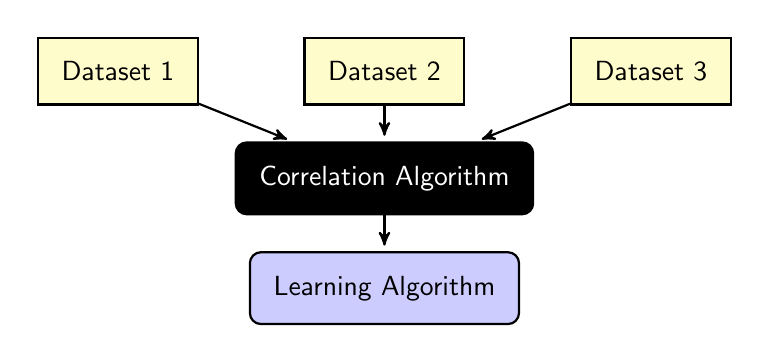
\begin{tikzpicture}[
      font=\sffamily,
      every matrix/.style={ampersand replacement=\&,column sep=3ex,row sep=3ex},
      dataset/.style={draw,thick,fill=yellow!20,inner sep=.3cm},
      sink/.style={dataset,rounded corners,fill=black, text=white},
      app/.style={dataset,rounded corners,fill=blue!20},
      dots/.style={gray,scale=2},
      to/.style={->,>=stealth',shorten >=2pt,thick,font=\sffamily\footnotesize},
      every node/.style={align=center}]

      \matrix{
        \node[dataset] (dataset1) {Dataset 1};
        \& \node[dataset] (dataset2) {Dataset 2};
        \& \node[dataset] (dataset3) {Dataset 3}; \\

        \& \node[sink] (blackbox) {Correlation Algorithm}; \& \\

        \& \node[app] (application) {Learning Algorithm}; \& \\      
      };

      \draw[to] (dataset1) -- (blackbox);
      \draw[to] (dataset2) -- (blackbox);
      \draw[to] (dataset3) -- (blackbox);
      \draw[to] (blackbox) -- (application);

    \end{tikzpicture}
  \end{center}

  \begin{center}
    \textbf{Goal}\\
    \vspace{1ex}
    \fcolorbox{black}[HTML]{F1F1F1}{\parbox{0.6\textwidth}{%
        \centering Develop theoretically justified, robust\\ correlation algorithms for\\
        multi-dataset fusion}}
  \end{center}

    
\end{frame}

\begin{frame}{A Myriad of Applications}

  \begin{columns}[T]
    \begin{column}{0.45\textwidth}
      
      \vspace{3ex}

      \textbf{Multiple Datasets}
      \begin{itemize}
      \item \textcolor<1>{texthigh}{Audio-Video}
      \item \textcolor<2>{texthigh}{Audio-Audio}
      \end{itemize}

      \hspace{2ex}
      

      \textbf{Machine Learning}
      \begin{itemize}
      \item \textcolor<3>{texthigh}{emotion identification}
      \item \textcolor<4>{texthigh}{shopping predictions}
      \item \textcolor<5>{texthigh}{music genre classification}
      \end{itemize}
      
      \hspace{2ex}

      \textbf{Medical Signal Processing}
      \begin{itemize}
      \item MRI, fMRi, EEG, MEG, etc.
      \end{itemize}


    \end{column}
    \begin{column}{0.45\textwidth}
      \begin{center}
      \includegraphics<1>[width=0.6\textwidth]{figures/parking_lot.jpg}\vspace{3ex}
      \includegraphics<1>[width=0.6\textwidth]{figures/car.png}
      \includegraphics<2>[width=0.8\textwidth]{figures/burton.jpg}
      \includegraphics<3>[width=0.6\textwidth]{figures/emotion1.png}
      \includegraphics<4>[width=0.8\textwidth]{figures/amazon_books.jpg}
      \includegraphics<5>[width=0.8\textwidth]{figures/Queen-Band.jpg}

      \vspace{4ex}

      \includegraphics<1>[width=0.6\textwidth]{figures/parking_lot2.jpg}
      \includegraphics<2>[width=0.8\textwidth]{figures/umich.png}
      \includegraphics<3>[width=0.7\textwidth]{figures/speaker_audio.pdf}
      \includegraphics<4>[width=0.8\textwidth]{figures/amazon_movies.jpg}
      \onslide<5>{\fcolorbox{black}[HTML]{F1F1F1}{\parbox{0.9\textwidth}{%
        \begin{itemize}
        \item disco influences
        \item danceable grooves
        \item repetitive melodic phrasing
        \item extensive vamping
        \item minor key tonality
        \end{itemize}}}}

  \end{center}
    \end{column}
  \end{columns}


\end{frame}


%%%%%%%%%%%%%%%%%%%%%%%%%%%%%%%%%%%%%%%%%%%%%%%%%%%%%%%%%%%%%%%%%%%%%%%%%%%%%%%%%%%%%%%%%%
\begin{frame}{Canonical Correlation Analysis}

  \textbf{What is it?}
  \begin{itemize}
  \item Dimensionality reduction algorithm for exactly 2 datasets, $X,Y$
  \item Correlation coefficients, linear transformations
  \end{itemize}

  \vspace{1ex}

  \textbf{What is it not?}
  \begin{itemize}
  \item Data fusion algorithm
  \end{itemize}
 

  \vspace{1ex}

  \begin{columns}
    \begin{column}{0.35\textwidth}
      \textbf{Covariance matrices}
      \begin{itemize}
      \item $\Rxx = \E{xx^H}$
      \item $\Ryy = \E{yy^H}$
      \item $\Rxy = \E{xy^H}$
      \end{itemize}
    \end{column}
    \begin{column}{0.55\textwidth}
      \begin{center}
        \textbf{Optimization problem}
        \vspace{-1ex}
        \begin{empheq}[box={\mybluebox[5pt][5pt][boxgrey]}]{equation*}
          \begin{aligned}
            & \argmax_{w_x,w_y} &&\rho = w_x^HR_{xy}w_y\\
            & \text{subject to } && w_x^H\Rxx w_x=1\\
            &&&w_y^H\Ryy w_y = 1\\
          \end{aligned}
        \end{empheq}
     \end{center}
    \end{column}
  \end{columns}

  \vspace{1ex}

  \textbf{Variable Transformation}
  \begin{itemize}
  \item $f=\Rxx^{1/2}w_x$
  \item $g=\Ryy^{1/2}w_y$
  \end{itemize}

\end{frame}

%%%%%%%%%%%%%%%%%%%%%%%%%%%%%%%%%%%%%%%%%%%%%%%%%%%%%%%%%%%%%%%%%%%%%%%%%%%%%%%%%%%%%%%%%%
\begin{frame}{Canonical Correlation Analysis}
  \addtocounter{framenumber}{-1}
  \textbf{What is it?}
  \begin{itemize}
  \item Dimensionality reduction algorithm for exactly 2 datasets
  \item Correlation coefficients, linear transformations
  \end{itemize}

  \vspace{1ex}

  \textbf{What is it not?}
  \begin{itemize}
  \item Data fusion algorithm
  \end{itemize}
 

  \vspace{1ex}

  \begin{center}
    \textbf{Optimization problem}
    \vspace{-1ex}
    \begin{empheq}[box={\mybluebox[5pt][5pt][boxgrey]}]{equation*}
      \begin{aligned}
        & \argmax_{f,g} &&\rho = f^H\,\underbrace{R_{xx}^{-1/2}R_{xy}R_{yy}^{-1/2}}_{\Ccca}g\\
        & \text{subject to } && \|f\|_2=1\,,\,\|g\|_2=1\\
      \end{aligned}
    \end{empheq}
  \end{center}


  \vspace{3ex}

  \begin{columns}[t]
    \begin{column}{0.3\textwidth}
      \textbf{Canonical Vectors}
      \begin{itemize}
      \item $w_x = R_{xx}^{-1/2}f$
      \item $w_y = R_{yy}^{-1/2}g$
      \end{itemize}
    \end{column}
    \begin{column}{0.4\textwidth}
      \centering
      \phantom{asdfas}\textbf{Insight}\\[-3ex]
      \begin{empheq}[box={\mybluebox[5pt][5pt][boxgrey]}]{equation*}
        \text{\# correlated signals $=k=\rank(\Ccca)$}
      \end{empheq}

    \end{column}
  \end{columns}

\end{frame}

%%%%%%%%%%%%%%%%%%%%%%%%%%%%%%%%%%%%%%%%%%%%%%%%%%%%%%%%%%%%%%%%%%%%%%%%%%%%%%%%%
\begin{frame}{Empirical CCA}

  \begin{columns}[t]
    \begin{column}{0.5\textwidth}

      \textbf{Training Datasets}
      \begin{itemize}
        \itemsep=1ex
      \item $X=\left[x_1,\dots,x_n\right]$
      \item $Y=\left[y_1,\dots,y_n\right]$
      \end{itemize}
    \end{column}
    \begin{column}{0.5\textwidth}

      \textbf{Sample Covariance Matrices}
      \begin{itemize}
      \item $\Rxxhat=\frac{1}{n}XX^H$
      \item $\Ryyhat=\frac{1}{n}YY^H$
      \item $\Rxyhat=\frac{1}{n}XY^H$
      \end{itemize}
    \end{column}
  \end{columns}

  \vspace{1ex}

  \begin{center}
    \textbf{Estimate}\\
    \fcolorbox{black}[HTML]{F1F1F1}{\parbox{0.4\textwidth}{%
        \be\ba
        &\Cccahat &&= \Rxxhat^{-1/2}\Rxyhat\Ryyhat^{-1/2}\\
        &&&=\widehat{F}\widehat{K}\widehat{G}^H
        \ea\ee
      }}
  \end{center}

      \textbf{Data SVDs}
      \begin{itemize}
        \itemsep=1ex
      \item $X = \Uxhat\Sigxhat\Vxhat^H$
      \item $Y=\Uyhat\Sigyhat\Vyhat^H$
      \item $\sigma\left(\Cccahat\right) = \sigma\left(\Vxhat^H\Vyhat\right)$
      \end{itemize}

\end{frame}

%%%%%%%%%%%%%%%%%%%%%%%%%%%%%%%%%%%%%%%%%%%%%%%%%%%%%%%%%%%%%%%%%%%%%%%%%%%%%%
\begin{frame}{Motivational Example -
    \href{run:/home/asendorf/Documents/thesis_videos/flashing_setup.mp4}{Flashing Light Video}}

  \begin{center}\textbf{Left Camera} \hspace{20ex} \textbf{Right Camera}\\
    \includegraphics[width=0.47\textwidth]{figures/flashing_left.png}\hspace{2ex}
    \includegraphics[width=0.47\textwidth]{figures/flashing_right.png}
  \end{center}

  \vspace{2ex}

  \textbf{System parameters}
  \begin{itemize}
  \item Vectorize $135\times 240$ image $\Rightarrow p=q=32400$ pixels
  \item 30 fps @ 30 seconds $\Rightarrow n=900$ frames
  \end{itemize}

  \begin{center}
  \textbf{Goal}\\
  \fcolorbox{black}[HTML]{F1F1F1}{\parbox{0.4\textwidth}{%
      \centering
      Identify correlated pixels between camera views
}}
\end{center}
  

\end{frame}

%%%%%%%%%%%%%%%%%%%%%%%%%%%%%%%%%%%%%%%%%%%%%%%%%%%%%%%%%%%%%%%%%%%%%%%%%%%%%%
\begin{frame}{\href{run:/home/asendorf/Documents/thesis_videos/flashing_cca.mp4}{Empirical
      CCA Results} -
    Canonical Vectors}

  \begin{itemize}
  \item After 900 frames = 30 seconds of video  
  \end{itemize}

  \begin{columns}
    \begin{column}{0.1\textwidth}
      \textbf{Left}\\
      \vspace{15ex}
      \textbf{Right}\\
    \end{column}
    \begin{column}{0.9\textwidth}
      \begin{center}
        \textbf{First} \hspace{15ex} \textbf{Second}\hspace{15ex}\textbf{Third}\\[1ex]
        \includegraphics[width=0.3\textwidth]{figures/flashing_cca_wx1.pdf}\hspace{1ex}
        \includegraphics[width=0.3\textwidth]{figures/flashing_cca_wx2.pdf}\hspace{1ex}
        \includegraphics[width=0.3\textwidth]{figures/flashing_cca_wx3.pdf}\\[2ex]
        \includegraphics[width=0.3\textwidth]{figures/flashing_cca_wy1.pdf}\hspace{1ex}
        \includegraphics[width=0.3\textwidth]{figures/flashing_cca_wy2.pdf}\hspace{1ex}
        \includegraphics[width=0.3\textwidth]{figures/flashing_cca_wy3.pdf}
      \end{center}
    \end{column}
  \end{columns}

\end{frame}

%%%%%%%%%%%%%%%%%%%%%%%%%%%%%%%%%%%%%%%%%%%%%%%%%%%%%%%%%%%%%%%%%%%%%%%%%%%%%%%%%%%%%%%%%%
\begin{frame}{Two-Dataset Model}

  \begin{center}
    \textbf{Linear Subspace Model\\}
    \vspace{0.5ex}
    \fcolorbox{black}[HTML]{F1F1F1}{\parbox{0.4\textwidth}{%
        \be\ba
        & x_i = \Ux\sx+\zx\\
        & y_i = \Uy\sy+\zy\\
        \ea\ee
      }}
  \end{center}

  \textbf{Parameters}
  \begin{itemize}
  \item $\Ux^H\Ux = I_{\kx}$, $\Uy^H\Uy = I_{\ky}$
  \item $\zx\simiid\mathcal{CN}(0,I_p)$, \,\,\,$\zy\simiid\mathcal{CN}(0,I_q)$
  \item
    $\E{\left[\begin{array}{c}\sx\\ \sy\end{array}\right]\left[\begin{array}{cc} \sx^H
          & \sy^H \end{array}\right]}= \left[\begin{array}{cc}\Tx & \Kxy\\
        \Kxy^H & \Ty \end{array}\right]$
  \item $\Kxy = \Tx^{1/2}\Pxy\Ty^{1/2}$
  \item $\Theta_x =
    \diag\left(\left(\theta_1^{(x)}\right)^2,\dots,\left(\theta_{k_x}^{(x)}\right)^2\right)$,\,\,\,
    $\Theta_y    =
    \diag\left(\left(\theta_1^{(y)}\right)^2,\dots,\left(\theta_{k_y}^{(y)}\right)^2\right)$  
  \item $\Pxy$ contains correlations $\rho_{kj}$ between signals of $\xii$ and $\yii$
  \item $\widetilde{K}_{xy}
    =\left(\Theta_x+I_{k_x}\right)^{-1/2}K_{xy}\left(\Theta_y+I_{k_y}\right)^{-1/2}$, with
    singular values $\kappa_1,\dots,\kappa_{\min(k_x,k_y)}$
  \end{itemize}
\end{frame}

%%%%%%%%%%%%%%%%%%%%%%%%%%%%%%%%%%%%%%%%%%%%
\begin{frame}{Informative CCA (ICCA)}


  \textbf{Not all singular vectors are informative!} (Nadakuditi, 2011)
  \begin{itemize}
  \item $\sigma_i\left(\Cccahat\right) = \sigma_i\left(\Vxhat^H\Vyhat\right)$
  \item Trim data SVD's to only use informative components
  \end{itemize}

  \vspace{2ex}

  \fcolorbox{black}[HTML]{F1F1F1}{\parbox{0.9\textwidth}{%
  \begin{enumerate}
    \itemsep=1ex
  \item Trim data SVD's: $X=\widehat{U}_x\,\widehat{\Sigma}_x\,\widehat{V}_x^H$ and $Y=\widehat{U}_y\,\widehat{\Sigma}_y\, \widehat{V}_y^H$
    \begin{itemize}
    \item $\Uxcir = \widehat{U}_x\left(:\,,1:\widehat{k}_x\right)$, $\Uycir = \widehat{U}_y\left(:\,,1:\widehat{k}_y\right)$
    \item $\Vxcir = \widehat{V}_x\left(:\,,1:\widehat{k}_x\right)$, $\Vycir = \widehat{V}_y\left(:\,,1:\widehat{k}_y\right)$
    \end{itemize}

  \item Form
    $\Ciccahat=\Uxcir\Vxcir^H\Vycir\Uycir$
  \item Take SVD: $\Ciccahat = \widetilde{F}\widetilde{K}\widetilde{G}^H$
  \item $\widehat{\rho}_{\text{icca}}^{(i)} = \widetilde{k}_i$
  \item $\widetilde{w}_x^{(i)}=\widehat{R}_{xx}^{-1/2}\,\widetilde{f}_i$
  \item $\widetilde{w}_y^{(i)}=\widehat{R}_{yy}^{-1/2}\,\widetilde{g}_i$
  \end{enumerate}}}

\end{frame}

%%%%%%%%%%%%%%%%%%%%%%%%%%%%%%%%%%%%%%%%%%%%%%%%%%%%%%%%%%%%%
\begin{frame}{New Algorithm: \iccap}

\textbf{Motivation}
\begin{itemize}
\item We expect ICCA to outperform CCA
\item However, we expect ICCA to be suboptimal because we substitute $\Uxhat$ and $\Uyhat$
  without considering accuracy
\end{itemize}

\vspace{2ex}

\begin{center}
  \textbf{Proposed Estimate}\\
  \fcolorbox{black}[HTML]{F1F1F1}{\parbox{0.7\textwidth}{%
      \be
      \widehat{w}_{x,i}^{\text{icca+}} = \Uxcir\diag\left(\lambda_{x,i}^{\text{opt}}\right)\Uktilhat\left(:,i\right)
      \ee
      \be
      \widehat{w}_{y,i}^{\text{icca+}} = \Uycir\diag\left(\lambda_{y,i}^{\text{opt}}\right)\Vktilhat\left(:,i\right),
      \ee
    }}
\end{center}  

\vspace{2ex}

\begin{center}
  \textbf{Optimization Problem}\\
  \fcolorbox{black}[HTML]{F1F1F1}{\parbox{0.7\textwidth}{%
\be
\lambda_{x,i}^{\text{opt}} = \argmin_{\lambda_x}\left\|w_x^{(i)} -
  \Uxhat\diag(\lambda_x)\Uktilhat\left(:,i\right)\right\|_F
\ee
\be
\lambda_{y,i}^{\text{opt}} = \argmin_{\lambda_y}\left\|w_y^{(i)} -
  \Uyhat\diag(\lambda_x)\Vktilhat\left(:,i\right)\right\|_F.
\ee}}
\end{center}

\end{frame}

%%%%%%%%%%%%%%%%%%%%%%%%%%%%%%%%%%%%%%%%%%%%%%%%%%%%%%%%%%
\begin{frame}{Closed Form Soluation}

\begin{prop}\label{prop:iccap}
The solutions to the previous optimization problem is given by
\begin{subequations}\label{eq:chpt5:can_opt_sol}
\be
\lambda_{x,i}^{\text{opt}} =
\diag\left(\Uxcir^H\Ux\left(\Tx+I_{\kx}\right)^{-1/2}\right)
\ee
\be
\lambda_{y,i}^{\text{opt}} =
\diag\left(\Uycir^H\Uy\left(\Ty+I_{\ky}\right)^{-1/2}\right).
\ee
\end{subequations}
\end{prop}

\vspace{2ex}

\textbf{Results from random matrix theory: Eigenvector accuracy}
\begin{center}
  \fcolorbox{black}[HTML]{F1F1F1}{\parbox{0.7\textwidth}{%
\be
|\langle\widehat{u}_i,u_i\rangle|^2\convas \begin{cases}
  \frac{-2\varphi_{\mu_Z}\left(\rho\right)}{\theta_i^2D^\prime_{\mu_Z}\left(\rho\right)}  
  &\theta_i^2>1/D_{\mu_Z}\left(b^+\right)\\ 0 & \text{otherwise}\end{cases} 
\ee}}\end{center}

\be
\ba
&D_{\mu}(z) \defeq
\left[\int\frac{z}{z^2-t^2}d_{\mu}(t)\right]\times\left[c_x\int\frac{z}{z^2-t^2}d_{\mu(t)}+
  \frac{1-c_x}{z}\right] \\
&\varphi_\mu\left(z\right) \defeq \int\frac{z}{z^2-t^2}d\mu\left(t\right)\\
\ea
\ee

\end{frame}


\begin{frame}{Main Theorem}
\begin{Th}
  The solution to the optimal \iccaps weights exhibits the following behavior
  in the asymptotic regime where $p,q,n\to\infty$ with $p/n\to c_x$ and $q/n\to c_y$.

  For $i=1,\dots,\kx$,
  \be
  \lambda_{x,\text{opt}}^{(i)} \convas 
  \begin{cases}
    D_{\mu_{Z_x}}\left(\sigma_x^{(i)}\right)\sqrt{\frac{-2\varphi_{\mu_{Z_x}}\left(\sigma_x^{(i)}\right)
      }{D^{\prime}_{\mu_{Z_x}}\left(\sigma_x^{(i)}\right)
        \left(1+D_{\mu_{Z_x}}\left(\sigma_x^{(i)}\right)\right)}} & \text{if }
    \left(\tx_i\right)^2 > 1/D_{\mu_{Z_x}}(b_x^+)\\ 
    0 & \text{otherwise} \\ \end{cases}
  \ee
  where $\sigma_x^{(i)}=D_{\mu_{Z_x}}^{-1}\left(1/\left(\tx_i\right)^2\right)$
and the  D-transform. A similar expression for
$\lambda_{y,\text{opt}}$ exists by replacing subscripts of $x$ with $y$. 
  \label{th:vect_opt}

\end{Th}

\vspace{3ex}

\textbf{Estimation using training data}
\begin{itemize}
\item Using data $X$, $Y$, we can estimate $\widehat{D}$, $\widehat{D}^\prime$,
  $\widehat{\varphi}_\mu$, and $\widehat{\varphi}_{\widetilde{\mu}}$
\end{itemize}

\end{frame}

%%%%%%%%%%%%%%%%%%%%%%%%%%%%%%%%%%%%%%%%%%%%%%%%%%%%%%%%%%%%%%%%%%%%%%%%%%%%%%
\begin{frame}{Canonical Vector Estimation}

\textbf{Data SVDs}
\begin{itemize}
\item $X=\Uxhat\Sigxhat\Vxhat^H$ with trimmed versions $\Uxcir$, $\Sigxcir$, $\Vxcir$
\item $\Uktil$ left singular vectors of $\Kxytil$
\item $\widehat{U}_{\widetilde{K}}$ left singular vectors of $\Cccahat$
\item $\Ukcir$ left singular vectors of $\Ciccahat$
\end{itemize}

\vspace{3ex}

\begin{table}[t]
\centering
\begin{tabular}{l|l}\toprule
Estimate & \\
\midrule
\textbf{Population}  & $W_x = \Ux\left(\Tx + I_{\kx}\right)^{-1/2}\Uktil$\\[1ex]
\textbf{Empirical CCA} & $\widehat{W}_x^{\text{cca}} =
\Uxhat\left(\Sigxhat\right)^{-1}\widehat{U}_{\widetilde{K}}$\\[1ex]
\textbf{ICCA} & $\widehat{W}_x^{\text{icca}} = \Uxcir\Sigxcir^{-1}\Ukcir$\\[1ex]
\textbf{\iccap} &$\widehat{W}_x^{\text{icca+}} = \Uxcir\Lambda_x^{\text{opt}}\Ukcir$\\[1ex]
\bottomrule
\end{tabular}
\end{table}

\end{frame}


%%%%%%%%%%%%%%%%%%%%%%%%%%%%%%%%%%%%%%%%%%%%%%%%%%%%%%%%%%%%%%%%%%%%%%%%%%%%%% 
\begin{frame}{Numerical Simulations}

\begin{itemize}
\item Rank-2 setting $\kx=\ky=2$, $p=200$, $q=250$, 
\item $\Tx=\Ty=\diag(16,4)$,  $\Pxy=\diag(0.9,0.5)$ 
\item Plot the accuracy of the first canonical vector for empirical CCA, ICCA, and \iccaps
\end{itemize}

\begin{figure}
  \subfigure[$n$ sweep]{
    \centering
    \includegraphics[width=0.3\textwidth]{figures/asilomar_n.pdf}  
  }
  \subfigure[$\theta$ sweep]{
    \centering
    \includegraphics[width=0.3\textwidth]{figures/asilomar_theta.pdf}  
  }
  \subfigure[$\widehat{k}$ sweep]{
    \centering
    \includegraphics[width=0.3\textwidth]{figures/khat_sweep.pdf}  
  }
\end{figure}


\end{frame}

%%%%%%%%%%%%%%%%%%%%%%%%%%%%%%%%%%%%%%%%%%%%%%%%%%%%%%%%%%%%%%%%%%%%%%%%%%%%%% 
\begin{frame}{\href{run:/home/asendorf/Documents/thesis_videos/flashing_video2.mp4}{Canonical Vector Accuracy Experiment}}

\begin{columns}[T]
  \begin{column}{0.3\textwidth}
    \vspace{15ex}
    \begin{center}
    \textbf{Original Scene}
    \includegraphics[width=\textwidth]{figures/flashing_left.png}
\end{center}
  \end{column}
  \begin{column}{0.7\textwidth}
    \begin{center}
      \textbf{ICCA}\hspace{20ex}\textbf{\iccap}\phantom{blah}\\
      \includegraphics[width=0.45\textwidth]{figures/flashing1_left1_icca.pdf}\hspace{2ex}
      \includegraphics[width=0.45\textwidth]{figures/flashing1_left1_opt.pdf}\\[2ex]
      \hspace{-2ex}\textbf{Empirical CCA}\hspace{13ex}\textbf{ICCA - \iccap}\\
      \includegraphics[width=0.45\textwidth]{figures/flashing1_left1_cca.pdf}\hspace{2ex}
      \includegraphics[width=0.45\textwidth]{figures/flashing1_left1_diff_icca.pdf}
    \end{center}
  \end{column}
\end{columns}
\end{frame}

%%%%%%%%%%%%%%%%%%%%%%%%%%%%%%%%%%%%
\begin{frame}{Conclusion}
  \begin{itemize}
  \item Improved canonical vector accuracy in low-sample, low-SNR regime in Canonical
    Correlation Analysis (CCA)
  \item Proposed a new algorithm: \iccap
  \item \iccap uses insights from random matrix theory to optimally scale sample
    eigenvectors 
    setting 
  \item \iccap is more robust to over estimation of number of signals
  \end{itemize}
\end{frame}

\end{document}
